\chapter{Music}
\section{Composition}
To create a sound accompaniment to the visual aspect we first need to consider
what style of music we should explore, that is to say, create at least an idea
of composition. Generative music is the technique we're exploring here, with
musical ideas being emergent from a set of parameters, and created from a system
that processes them. The definition is fairly vague as with generative art, the
main requirement is that a system is setup and creates the music, this doesn't
need to be a computer, but often is.

Generative music is rather recent, with Brian Eno being major figure
popularising its use, he would often use the analogy of a Moir\'{e} pattern to
describe how the programs would work at the time.  

The immediate style of music to draw from Viner's work would probably be that of
minimalism, the repetition and difference across an image is very similar in
style to especially the percussive works of Reich, Glass, Riley, and even the
drone works of La Monte Young to an extent. Another, less famous example that I
feel conveys the feeling well is \emph{Jon Gibson - Cycles (1977)}, the cover
for the recording is a Moir\'{e} pattern, and the work modulates a 7-note
pattern that comes into and out of phase with itself. 

In fact, Eno refers to his inspiration of generative music to be triggered by
hearing \emph{It's Gonna Rain} by Reich, linking generative music as a concept
pretty solidly to Minimalism. Reich used the analogy of fabric work and weaving,
featuring on the cover of Music for 18 Musicians is a woven piece of fabric;
this seems similar to the idea of a grid (given that weaving takes place on a
matrix of strings, perhaps the crossing points could be seen as `vertices')

There is also a nice parallel from the graphical scores of Xenakis to Viner's
works, at least aesthetically (see \autoref{xevicompare}). Xenakis is the
so-called `father of granular synthesis', this technique is made of playing many
small, short sounds (grains) to create what is often described as a `cloud' of
sound. Xenakis was also a pioneer of ideas of stochasticism in music and could
be said to be one of the first generative composers in that respect. 

\begin{figure}
    \centering
    \begin{subfigure}[t]{.49\textwidth}
        \centering
        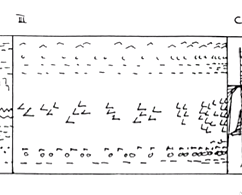
\includegraphics[width=.7\linewidth]{metastasis-3}
        \caption*{\emph{Movement 3 of Xenakis' Metastasis}}
    \end{subfigure}
    \begin{subfigure}[t]{.49\textwidth}
        \centering
        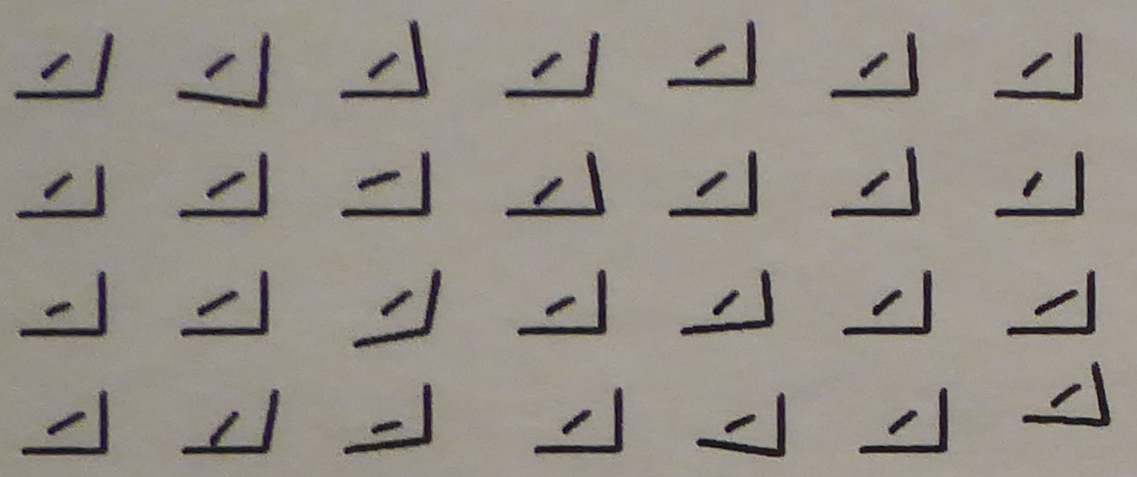
\includegraphics[width=.7\linewidth]{viner2}
        \caption*{\emph{Darrell Viner, Untitled (1974)} \copyright Victoria and
    Albert Museum, London.}
    \end{subfigure}
    \caption{Comparison of Xenakis and Viner}
    \label{xevicompare}
\end{figure}


Overall the idea with the composition should be to enhance what is on the
screen, if the image is disordered the sound should be too, if it is ordered
and regular the sound should follow. 

An idea here is to use a kernel or convolution matrix to be able to take the
whole image's current parameters for each element in the grid and map it down to
a smaller dataset for use as parameters to the synthesiser, essentially
downscaling the image. This could be used powerfully with the idea of granular
synthesis as, for example each parameter could change something about a grain
(playback speed, volume, effect intensity). This feels also almost like the
feeling of the Moir\'{e} pattern mentioned by Eno. 

Further this will be combined with the methods mentioned in
\autoref{sonicnav}, including the ideas present in the mentioned minimalist
composers.

\section{Synthesis}
There are many options for digital synthesis of which I've already mentioned
granular synthesis, but frequency modulation, additive, wavetable, modal, and so
on are also options.

Largely there are four approaches, that of the Processed Recording, the Spectral
Model, the Physical Model, and the Abstract Algorithm \citep{smith_2005}.

For this project spectral and physical modelling are out of the scope and would
require more specialist audio software frameworks. Processed recording, includes
more sample-based audio and manipulation of that, granular synthesis is an
example. The 'abstract algorithm' methods include things like FM synthesis,
which in its most basic form is comprised of a carrier waveform who's frequency
is modulated by another waveform, this can be extended by things like including
feedback at various stages of the processing.

On top of these methods, there should also be a consideration to audio effects,
processing and p5.js both have sound libraries with built-in audio effects,
reverb and delay perhaps being the most important to create the idea of a space
in the sound.

Creating these methods in software are fairly straightforward when there is
already some digital signal processing in place; p5.js has a library called
\verb|Tone.JS| which handles a lot of the practical elements of sound
generation.
